% ============================================================================
% aoi-micro — информационная база / черновик статьи
% Источники: README.md, docs/INTERVIEW.md, bench/RESULTS.md, nn_results/det_v0/
% Оформление: нейтральный article; легко перенастроить под требования редакции.
% Сборка: pdflatex main.tex  (или latexmk -pdf main.tex)
% ============================================================================
\documentclass[12pt,a4paper]{article}

\usepackage[T2A]{fontenc}
\usepackage[utf8]{inputenc}
\usepackage[russian,english]{babel}
\usepackage{geometry}
\geometry{margin=2.2cm}
\usepackage{graphicx}
\usepackage{booktabs}
\usepackage{tabularx}
\usepackage{multirow}
\usepackage{amsmath,amssymb}
\usepackage{siunitx}
\usepackage{hyperref}
\usepackage{xcolor}
\usepackage{enumitem}
\usepackage{caption}
\usepackage{subcaption}
\usepackage{float}
\usepackage{csquotes}
\usepackage{microtype}

\hypersetup{
  colorlinks=true,
  linkcolor=black,
  citecolor=black,
  urlcolor=blue!50!black
}

\title{CAD-управляемый прототип 2D~AOI\\
\large классический пайплайн OpenCV и опциональный детектор компонентов}
\author{Иван Илюхин\\
\textit{Applied AI / Computer Vision / Python}\\
\texttt{github.com/f1b0nacc1-afk/aoi-micro}}
\date{черновик информационной базы --- \today}

\begin{document}
\maketitle

\begin{abstract}
\noindent
Документ фиксирует постановку, обоснование, методы и численные результаты
проекта \textbf{aoi-micro}: прототип оптической инспекции печатных плат (AOI)
для одной верхней монохромной камеры. Основной продукт --- \emph{классический}
пайплайн (фидуциалы, CAD-окна, вариационная golden-модель, PASS/FAIL),
в духе промышленных variation-model систем. Нейросетевой детектор YOLO11s
рассматривается только как исследовательский эксперимент <<второго мнения>>,
не как заявка на линейную инспекцию. Метрики классического контура получены
на \textbf{синтетическом стенде} (v6: обнаружение дефектов \(93{,}3\,\%\),
верный класс \(87{,}6\,\%\), \(0\,\%\) брака как PASS); метрики детектора ---
на синтетике (mAP50 \(0{,}93\)) и публичных фото (mAP50 \(0{,}38\)).
\end{abstract}

\tableofcontents
\newpage

%--------------------------------------------------------------------------
\section{Назначение документа}
%--------------------------------------------------------------------------

Этот файл --- \textbf{информационная база} для будущей статьи / отчёта.
Структура уже близка к исследовательской публикации: мотивация, методы,
эксперимент, результаты, ограничения. Когда появятся требования редакции
(шаблон, язык, объём, стиль ссылок), достаточно заменить преамбулу и
перенести разделы.

\textbf{Источники фактов в репозитории:}
\begin{itemize}[leftmargin=1.5em,itemsep=0.2em]
  \item \texttt{README.md} --- позиционирование и сводка метрик;
  \item \texttt{docs/INTERVIEW.md} --- аргументация classical vs YOLO;
  \item \texttt{bench/RESULTS.md} --- журнал прогонов v0--v6 и holdout;
  \item \texttt{nn\_results/det\_v0/} --- обучение и eval детектора;
  \item код: \texttt{aoi/align.py}, \texttt{model.py}, \texttt{inspect.py},
        \texttt{optics.py}, \texttt{aoi/nn/*}, \texttt{aoi/bench/*}.
\end{itemize}

\textbf{Честная рамка:} прототип, не внедрённая линия; бэкенды Basler/Hikrobot
следуют API производителей, но \emph{не верифицированы на железе}; все
KPIs стенда --- синтетические, не заводской OEE/SLA.

%--------------------------------------------------------------------------
\section{Введение и мотивация}
%--------------------------------------------------------------------------

\subsection{Задача}
Автоматическая оптическая инспекция (AOI) после SMT: для каждой позиции
BOM/centroid проверить наличие, сдвиг, поворот/полярность, грубые паяные
и поверхностные аномалии; выдать PASS/FAIL с кропами и машиночитаемым
отчётом (CSV/JSON/HTML).

Целевой контур съёмки: одна верхняя камера (ориентир --- IMX183 + Computar
\(12\,\mathrm{mm}\); в коде --- бэкенды Basler acA5472-17um /
Hikrobot MV-CE200-10UM), фиксированная экспозиция и диафрагма, кольцевой
или купольный свет (коаксиал на широком поле со крутыми углами лучей
обычно проигрывает).

\subsection{Почему классика, а не <<только YOLO>>}
\begin{enumerate}[leftmargin=1.5em]
  \item При известном CAD и контролируемой оптике задача ближе к
        \emph{метрологии + таксономии дефектов}, чем к open-world detection.
  \item Детектор даёт класс и рамку, но слабо отвечает на
        <<нормален ли паяный шов / полярность / допуск сдвига в мм>>
        без отдельных голов и разметки.
  \item Смена партии корпусов (оттенок, дата-код) при чистом appearance-модели
        требует дообучения; вариационная зональная модель допускает
        явную политику <<тело vs выводы>>.
  \item NCC alone контрастно-инвариантна и может <<найти>> деталь на пустых
        площадках с похожей геометрией зазоров --- нужен фотометрический
        контур (MAD, тон корпуса).
\end{enumerate}

\textbf{Позиционирование проекта:} industrial 2D~AOI без обязательного DL,
когда геометрия, свет и golden-партия под контролем --- та же идея
variation model, что в промышленных инструментах (в т.\,ч.\ стиль
MVTec HALCON), реализованная на OpenCV. YOLO --- опциональный эксперимент.

%--------------------------------------------------------------------------
\section{Смежные подходы и обоснование выбора}
\label{sec:related}
%--------------------------------------------------------------------------

\begin{table}[H]
\centering
\caption{Сравнение парадигм в контексте данного прототипа}
\label{tab:paradigms}
\begin{tabular}{@{}p{3.2cm}p{5.8cm}p{5.8cm}@{}}
\toprule
 & \textbf{Classical (aoi-micro)} & \textbf{YOLO-детектор} \\
\midrule
Prior & CAD + библиотека корпусов + golden-партия
      & размеченные боксы, выученный внешний вид \\
Выход & PASS/FAIL по refdes, сдвиг/полярность/припой в измеримых признаках
      & класс + box; <<шов OK?>> без доп.\ голов слабо \\
Смена партии & зонная модель (inner vs border)
             & retrain / domain adaptation \\
Пустая площадка & photometric MAD + тон ломают неоднозначность NCC
                 & класс footprint/empty и достаточная выборка \\
Где выигрывает & контролируемая оптика, известный BOM, есть golden
                & плотный clutter, нет CAD, open-world номенклатура \\
\bottomrule
\end{tabular}
\end{table}

Практический вывод для статьи: классический контур --- основной метод;
детектор --- second opinion (пустой слот / чужое семейство) или путь
при отсутствии CAD.

%--------------------------------------------------------------------------
\section{Оптика и геометрия}
\label{sec:optics}
%--------------------------------------------------------------------------

\subsection{Масштаб и рабочая дистанция}
Модуль \texttt{aoi/optics.py} считает поле, \(\mathrm{\mu m/px}\), ГРИП и
параллакс для фиксированного фокуса. WD измеряется от передней линзы;
смещение к главной плоскости (\(\approx 27\,\mathrm{mm}\) для воспроизведения
каталожного поля Computar V1226-MPZ при MOD \(100\,\mathrm{mm}\)).

\subsection{Параллакс высоких корпусов}
Центр CAD-окна для детали высоты \(h\) на расстоянии \(r\) от оптической оси
смещается:
\begin{equation}
  \Delta \approx \frac{r \cdot h}{\mathrm{WD}-h}.
\end{equation}
Неверный WD систематически смещает окна и выглядит как <<глобальный shift>>.
Допуск \texttt{edge\_tol\_mm} должен лежать выше разброса установки
(\(\sim 2\)--\(3\sigma\)) и ниже половины шага выводов: при
\(\sim 23\,\mathrm{\mu m/px}\) (WD \(100\)) мост на шаге \(0{,}8\,\mathrm{mm}\)
ловим; при \(\sim 45\,\mathrm{\mu m/px}\) --- уже нет.

\subsection{Калибровка}
ChArUco: \texttt{calib-target} \(\to\) съёмка \(\to\) \texttt{calibrate}
\(\to\) \texttt{camera.npz}/\texttt{camera.json}. Проверка на синтетике:
\texttt{tests/test\_calib.py}.

%--------------------------------------------------------------------------
\section{Методы: классический пайплайн}
\label{sec:classical}
%--------------------------------------------------------------------------

Пайплайн (рис.~логически: Align \(\to\) CAD windows \(\to\) Golden \(\to\)
Inspect \(\to\) Report).

\subsection{Выравнивание (Align)}
Фидуциалы \(\to\) система платы с фиксированным \(\mathrm{px/mm}\):
\begin{itemize}[leftmargin=1.5em,itemsep=0.15em]
  \item 2 фидуциала --- similarity;
  \item 3 --- affine;
  \item \(\ge 4\) --- homography.
\end{itemize}
Уточнение ECC относительно среднего golden; низкочастотная нормализация
освещённости.

\subsection{CAD-окна}
Файл центроидов (KiCad \texttt{.pos}, Altium Pick\&Place, CSV) + библиотека
корпусов \(\to\) окно на каждую посадку; центр сдвинут на параллакс
(см.~\ref{sec:optics}).

\subsection{Golden-модель}
По \(\sim 20\)--\(30\) заведомо годным платам партии~A: попозиционные
mean/\(\sigma\), распределения NCC и фотометрического MAD. Пороги --- из
статистики, не ручные константы.

\subsection{Зональная модель корпуса (ключевой инсайт)}
\begin{description}[leftmargin=1.2em,style=nextline]
  \item[Внутренняя зона] маркировка и тон партии --- медиана с допуском
        \(\texttt{body\_tol\_abs} + \texttt{body\_tol\_rel}\cdot\mathrm{median}\)
        (игнорировать вариацию дата-кода/краски).
  \item[Рамка / выводы] mean absolute difference vs golden после компенсации
        локального сдвига яркости.
\end{description}
NCC alone недостаточна: наличие требует \textbf{NCC \(\land\) border MAD
\(\land\) inner tone}. Зоны обрушили ложные срабатывания на синтетической
партии~B с \(61{,}1\,\%\) (v0) до \(\sim 0{,}6\)--\(1\,\%\) (v6).

\subsection{Инспекция}
\begin{itemize}[leftmargin=1.5em,itemsep=0.2em]
  \item поиск сдвига/поворота шаблоном NCC (\(\pm 0{,}8\,\mathrm{mm}\),
        \(\pm 20^\circ\)); позиция ограничена \texttt{search\_mm}, иначе
        широкий поиск;
  \item сдвиг выше допуска при уверенном match \(\to\) SHIFT, не MISSING;
        потолок допуска \texttt{shift\_tol\_max\_mm} \(= 0{,}5\,\mathrm{mm}\);
  \item полярность: поиск golden-метки (pin~1, полоска диода, <<\(-\)>>
        электролита) в 4 ориентациях (квадрат) или 2 (двусторонние
        полярные); fallback --- перевёрнутый шаблон;
  \item верхняя грань: отклонение от golden после компенсации тона
        (сколы/царапины);
  \item припой: доля пикселей зоны выводов с \(z > 2{,}5\)
        (\texttt{joint\_frac}; на хороших \(\le 0{,}030\), на непропае
        \(\ge 0{,}078\) в пробе v5);
  \item пятна вне деталей: вариационная модель экстерьера платы.
\end{itemize}

\subsection{Отчёт}
PASS/FAIL по позиции; кропы live\,|\,golden\,|\,deviation; CSV/JSON/HTML.

%--------------------------------------------------------------------------
\section{Методы: синтетический стенд}
\label{sec:bench}
%--------------------------------------------------------------------------

Модуль \texttt{aoi bench} строит процедурные платы: маска, трассы, корпуса,
параллакс, дефокус, виньетка, поза, шум сенсора; размеченные типы дефектов.
Протокол (v6, 2026-10-07):
\begin{itemize}[leftmargin=1.5em]
  \item 4 дизайна \(\times\) (20 golden + 2 good~A + 2 good~B + 4 бракованных
        по 6 дефектов) \(=\) \textbf{89} размеченных дефектов,
        \(\approx 2000\) позиций инспекции;
  \item партия~B: другие оттенки корпусов, маркировка/дата-коды, без следа
        эжектора;
  \item holdout \texttt{seed~7}: другие 4 дизайна, на которых пороги не
        подбирались.
\end{itemize}

\begin{figure}[H]
\centering
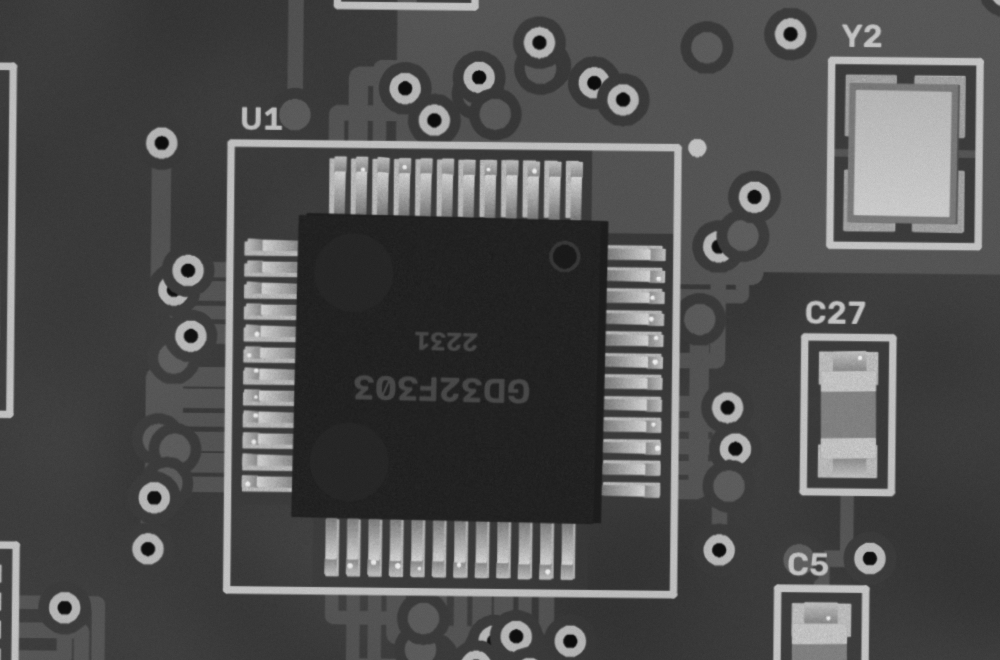
\includegraphics[width=0.72\textwidth]{figures/bench_preview.png}
\caption{Пример синтетического кадра стенда (превью LQFP-дизайна).}
\label{fig:bench}
\end{figure}

Метрики: detection rate, accuracy класса дефекта, bad-as-PASS, false
positions на good~A/B, доля good-плат с FAIL. Разбор промахов:
\texttt{python -m aoi.bench.analyze}.

\textbf{Не цитировать как заводской KPI.}

%--------------------------------------------------------------------------
\section{Результаты: классический AOI}
\label{sec:res-classical}
%--------------------------------------------------------------------------

\begin{table}[H]
\centering
\caption{Синтетический стенд: эволюция v0\(\to\)v6 и holdout
(\texttt{bench/RESULTS.md})}
\label{tab:v6}
\begin{tabular}{@{}lcccc@{}}
\toprule
Метрика & v0 & v1 zones & \textbf{v6} & v6 holdout \\
\midrule
Обнаружение дефектов, \%
  & 76{,}4 & 88{,}8 & \textbf{93{,}3} & \textbf{93{,}3} \\
Верный класс дефекта, \%
  & 59{,}6 & 71{,}9 & \textbf{87{,}6} & 84{,}3 \\
Брак как PASS, \%
  & 0 & 0 & 0 & 0 \\
Ложные поз., good A, \%
  & 0{,}8 & 0{,}4 & 0{,}6 & 1{,}4 \\
Ложные поз., good B, \%
  & \textbf{61{,}1} & 0{,}6 & 0{,}8 & 1{,}2 \\
Train / inspect платы, с
  & 80 / 3{,}2 & 21 / 1{,}5 & 22 / 1{,}6 & 22 / 1{,}5 \\
\bottomrule
\end{tabular}
\end{table}

\subsection{Что изменили (v1--v6)}
\begin{enumerate}[leftmargin=1.5em,itemsep=0.15em]
  \item Зоны корпуса --- главный эффект на партии~B.
  \item Надёжный поиск полярности (4/2 ориентации + fallback).
  \item Политика SHIFT vs MISSING и потолок допуска сдвига.
  \item Верхнегранные дефекты после компенсации тона.
  \item \texttt{joint\_frac} для непропая / аномалий шва.
  \item Пятна на плате в полном разрешении; атрибуция к соседнему грубому
        дефекту.
  \item Грубый\(\to\)точный угол при обучении: train \(\times 3{,}6\) быстрее.
\end{enumerate}

\subsection{Отброшенные идеи}
Отношение градиентов по контуру не отличает тёмный missing на тёмной маске;
медиана яркости площадок давала шум \(\pm 15\)--\(24\) на хороших платах.

\subsection{Слабые места (честно в статью)}
\begin{itemize}[leftmargin=1.5em,itemsep=0.15em]
  \item \textbf{damaged} на светлых выводах --- нужен косой/кольцевой свет
        или 2-й ракурс;
  \item \textbf{marking} / подмена IC той же формы --- только OCR (нет);
  \item \textbf{excess} часто как MISMATCH/MISSING при \(100\,\%\) detection;
  \item SOT-23: отсутствие/переворот как ANOMALY (класс неверный);
  \item false positions \(\sim 0{,}6\)--\(1{,}4\,\%\) vs цель линии \(<0{,}2\,\%\);
        при \(\sim 65\) деталях на плату даже \(1\,\%\) даёт FAIL на большой
        доле <<хороших>> плат (31--69\,\% плат с FAIL при низком per-position
        FP).
\end{itemize}

\subsection{Покрытие дефектов (v6 / holdout), кратко}
Хорошо: missing, shift, polarity, rot90, wrong, tombstone, billboard,
no\_solder, bridge, ball, foreign. Слабее: damaged, marking (OCR-only),
часть excess по классу.

%--------------------------------------------------------------------------
\section{Эксперимент: нейросетевой детектор}
\label{sec:nn}
%--------------------------------------------------------------------------

\subsection{Постановка}
Опциональный путь \texttt{aoi/nn/}: YOLO11s, единый набор классов
(\texttt{resistor}, \texttt{capacitor}, \texttt{electrolytic}, \texttt{ic},
\texttt{transistor}, \texttt{diode}, \texttt{led}, \texttt{inductor},
\texttt{crystal}, \texttt{footprint}, \texttt{other}), обучение на
публичных датасетах + синтетике стенда. Роль --- second opinion /
research, не заявленная линейная инспекция.

Типичный запуск (фактически det\_v0: 40 эпох, imgsz 1024):
\begin{verbatim}
python -m aoi.nn.train --data data/yolo/public data/yolo/synth --name det_v0
python -m aoi.nn.evaluate runs/nn/det_v0/weights/best.pt
\end{verbatim}

\subsection{Обучение}
По \texttt{nn\_results/det\_v0/results.csv}: 40 эпох; к концу
mAP50 \(\approx 0{,}544\), mAP50-95 \(\approx 0{,}428\), recall \(\approx 0{,}53\),
precision \(\approx 0{,}77\) (агрегат по смешанной валидации). Losses
(box/cls/dfl) монотонно снижаются на train и val.

\begin{figure}[H]
\centering
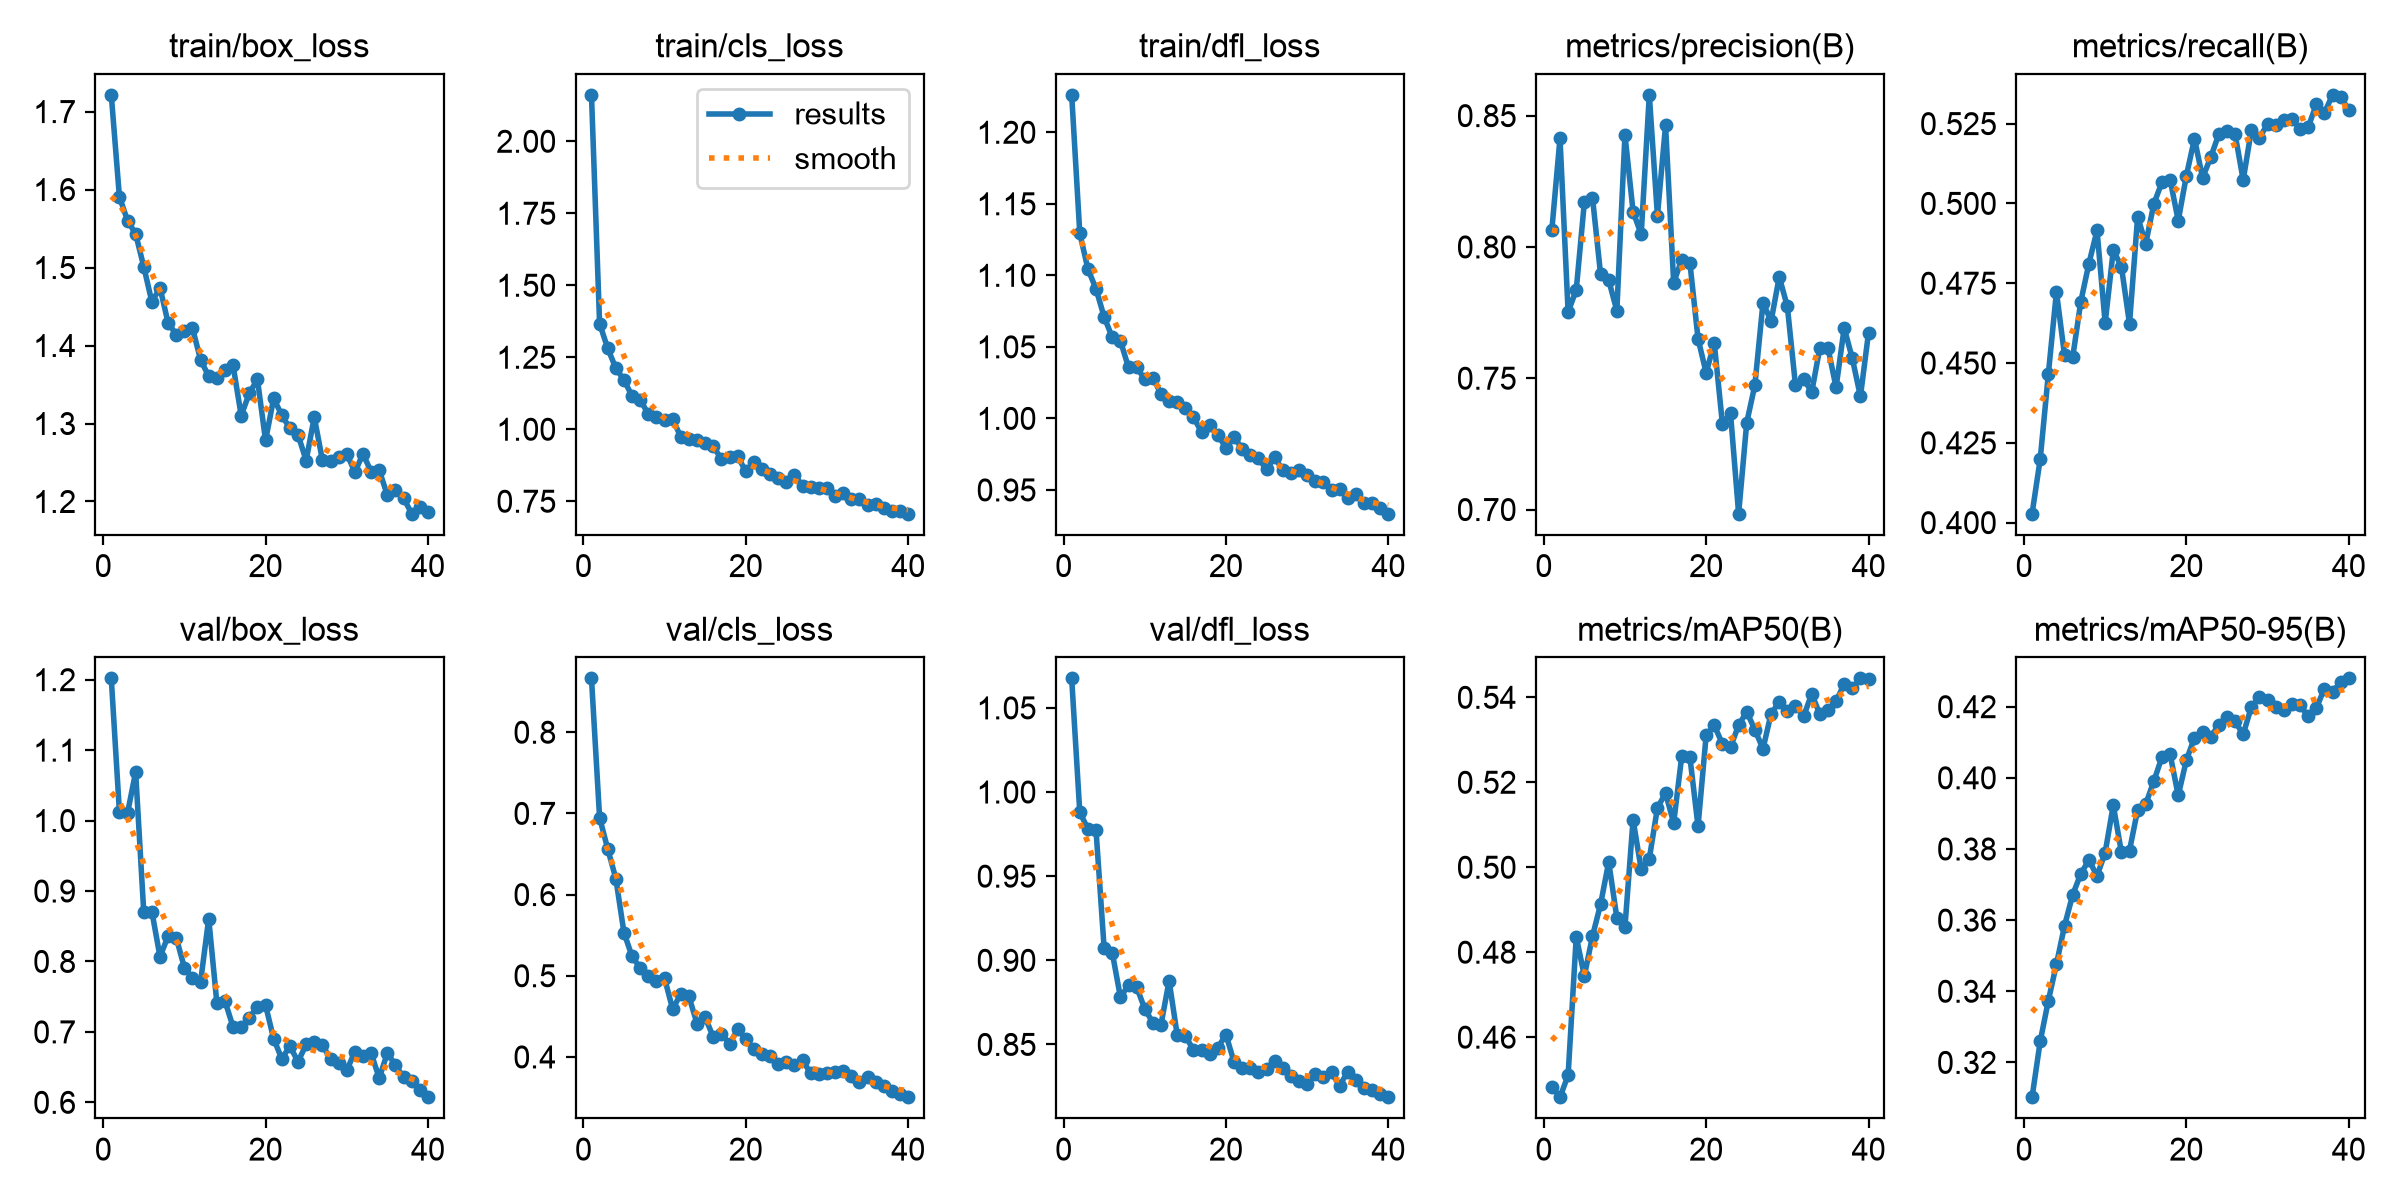
\includegraphics[width=\textwidth]{figures/results.png}
\caption{Кривые обучения YOLO11s (det\_v0): losses, precision, recall, mAP.}
\label{fig:train}
\end{figure}

\begin{figure}[H]
\centering
\begin{subfigure}[t]{0.48\textwidth}
  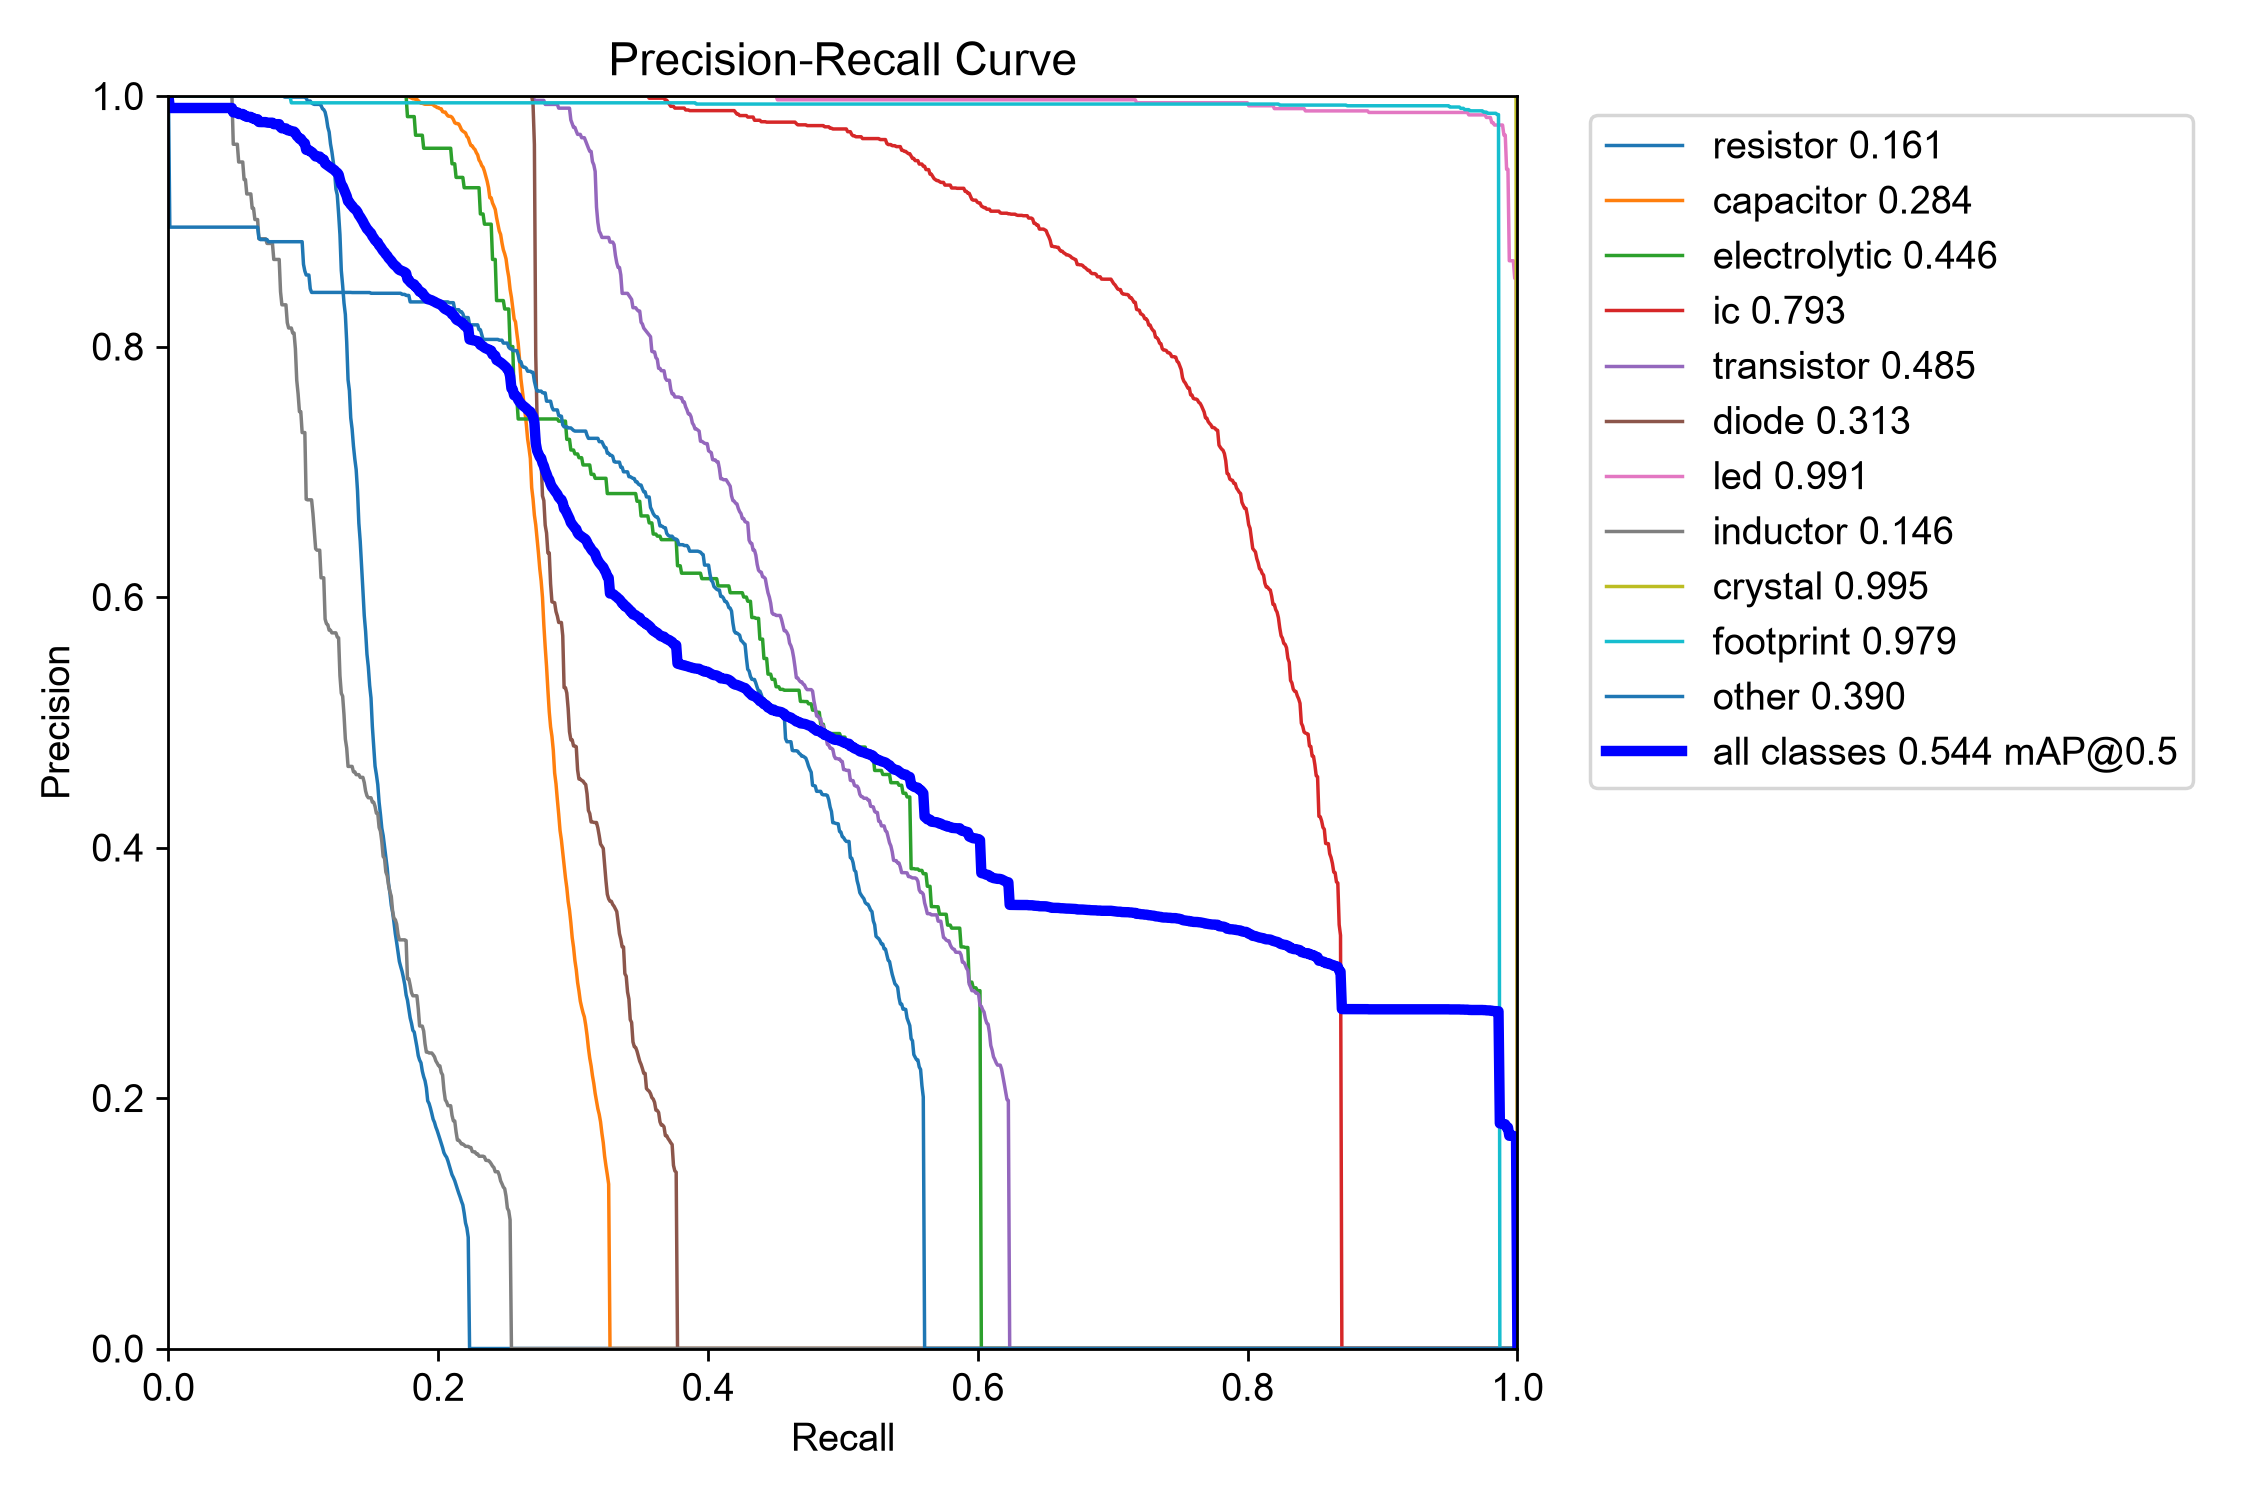
\includegraphics[width=\linewidth]{figures/BoxPR_curve.png}
  \caption{PR-кривые (Box), mAP@0.5 по классам.}
\end{subfigure}\hfill
\begin{subfigure}[t]{0.48\textwidth}
  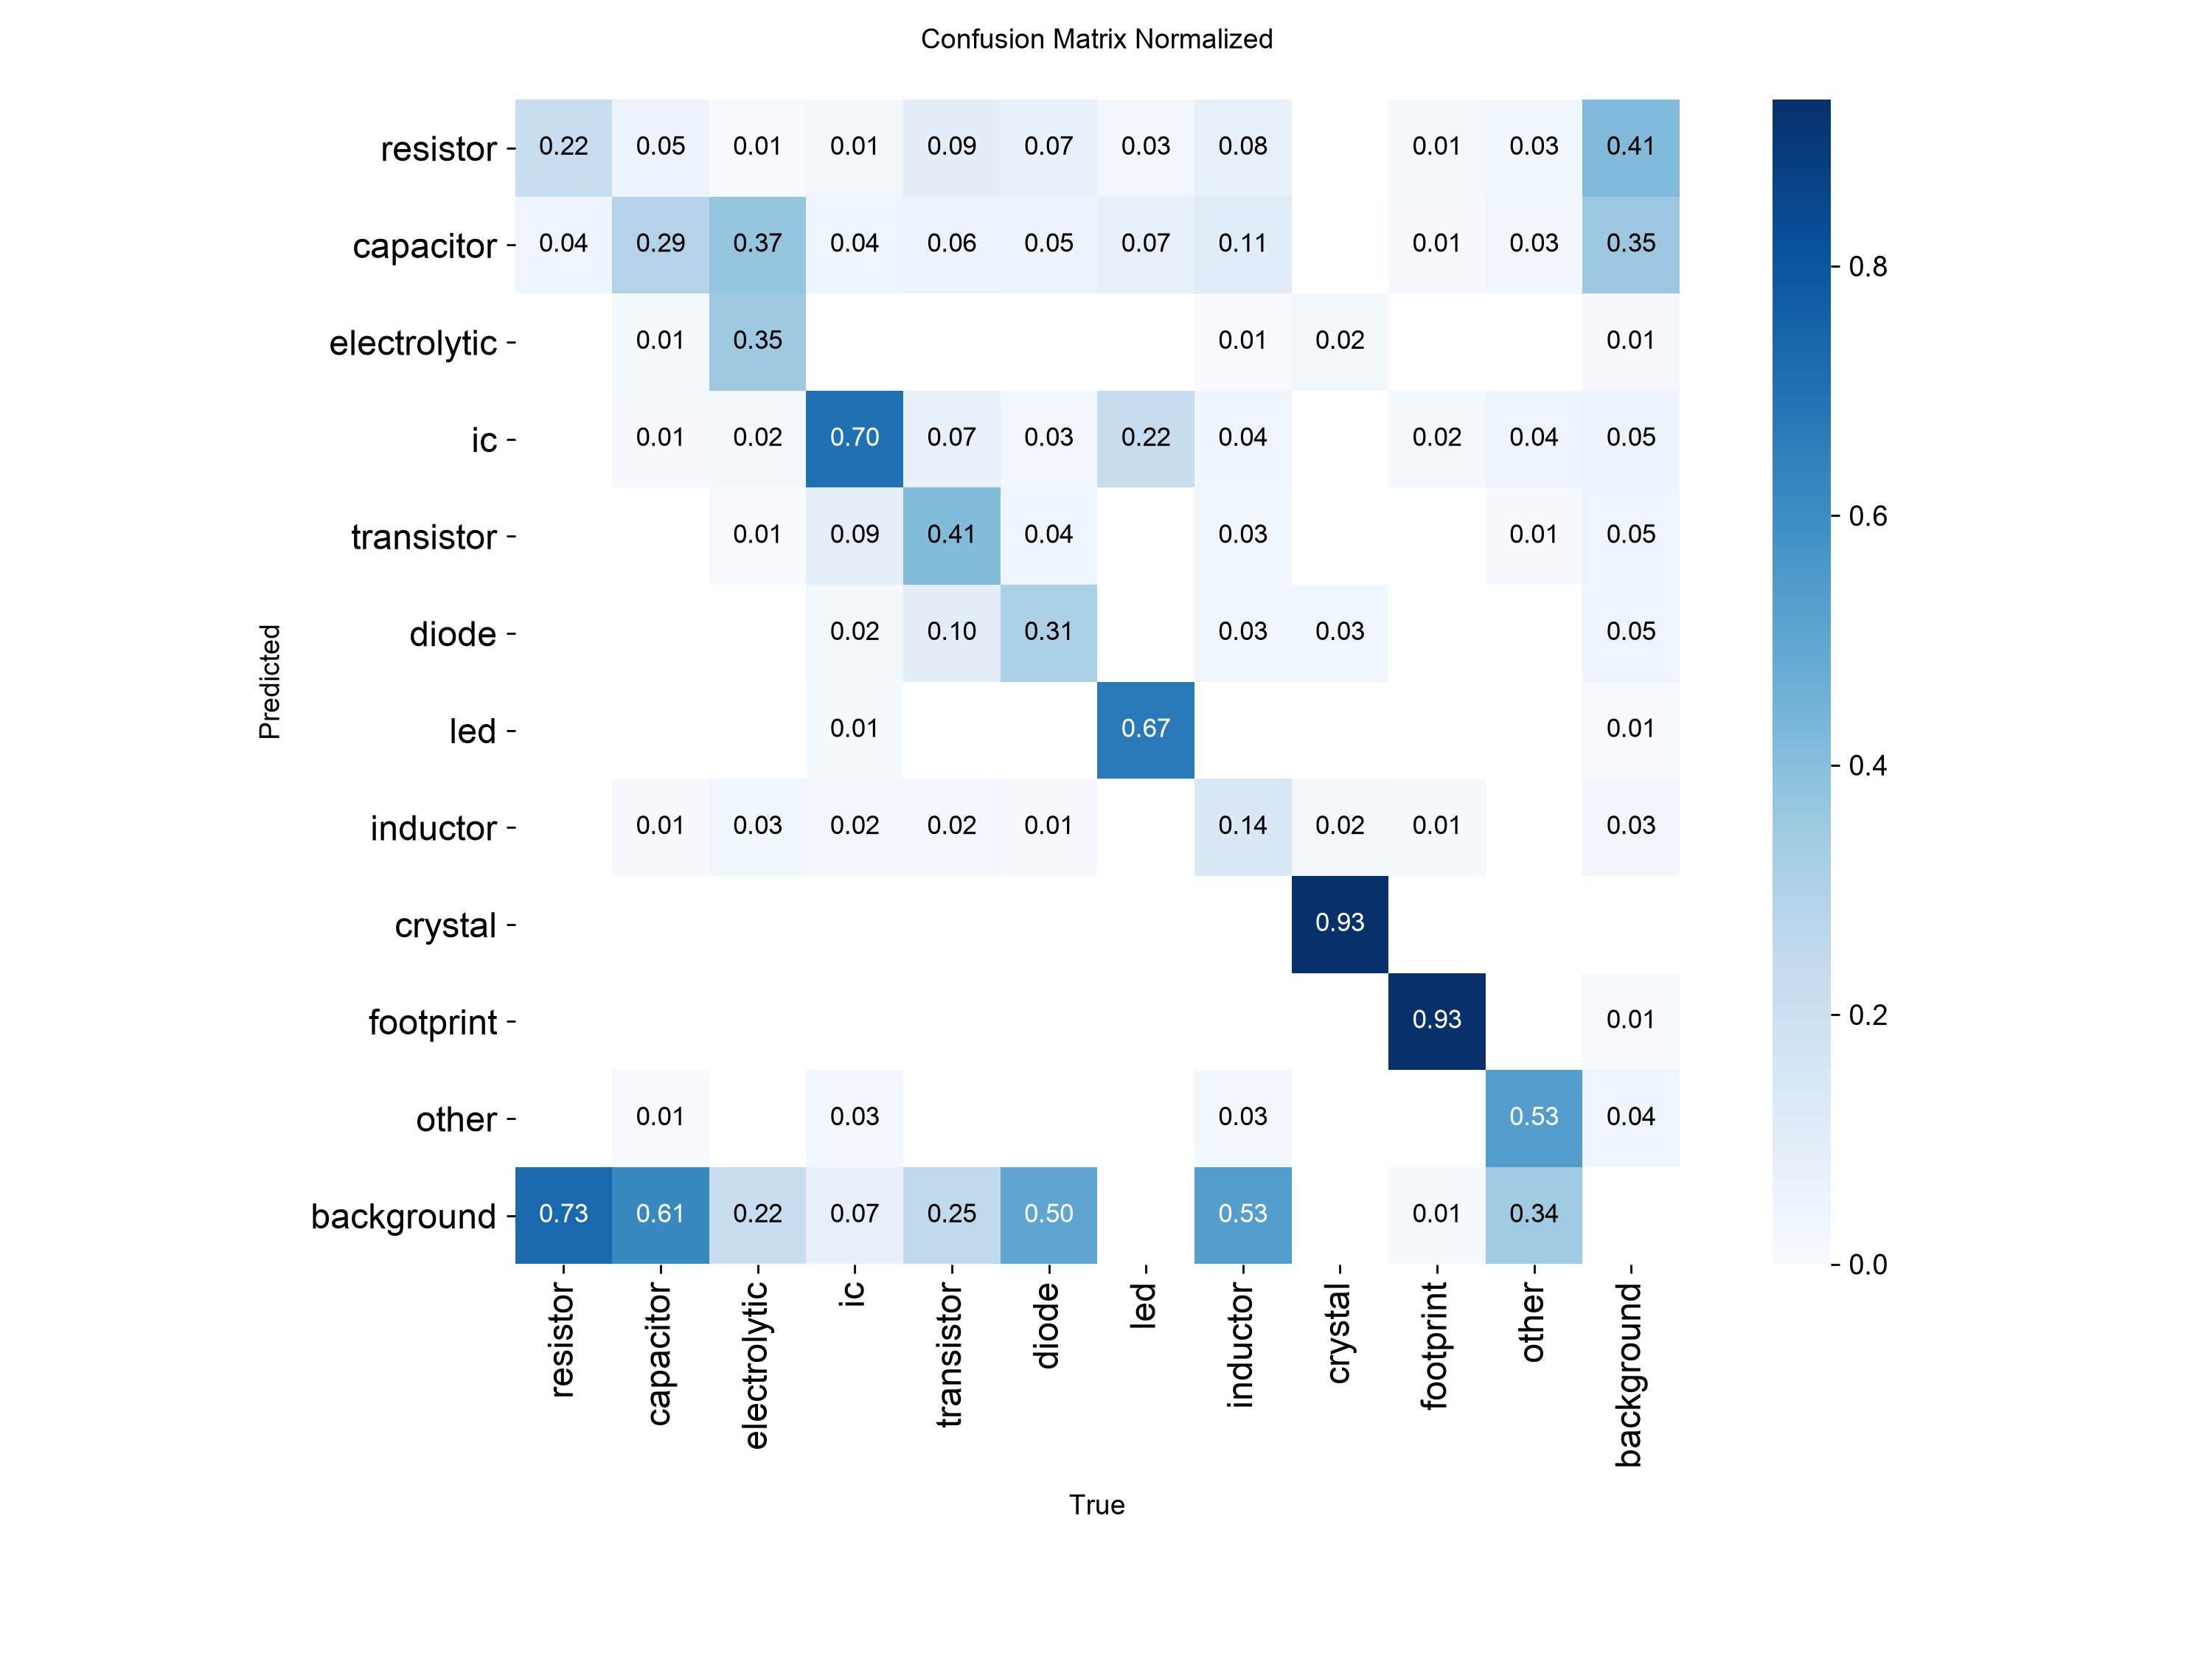
\includegraphics[width=\linewidth]{figures/confusion_matrix_normalized.png}
  \caption{Нормализованная confusion matrix.}
\end{subfigure}
\caption{Диагностика классификации/детекции на валидации.}
\label{fig:pr-cm}
\end{figure}

\begin{figure}[H]
\centering
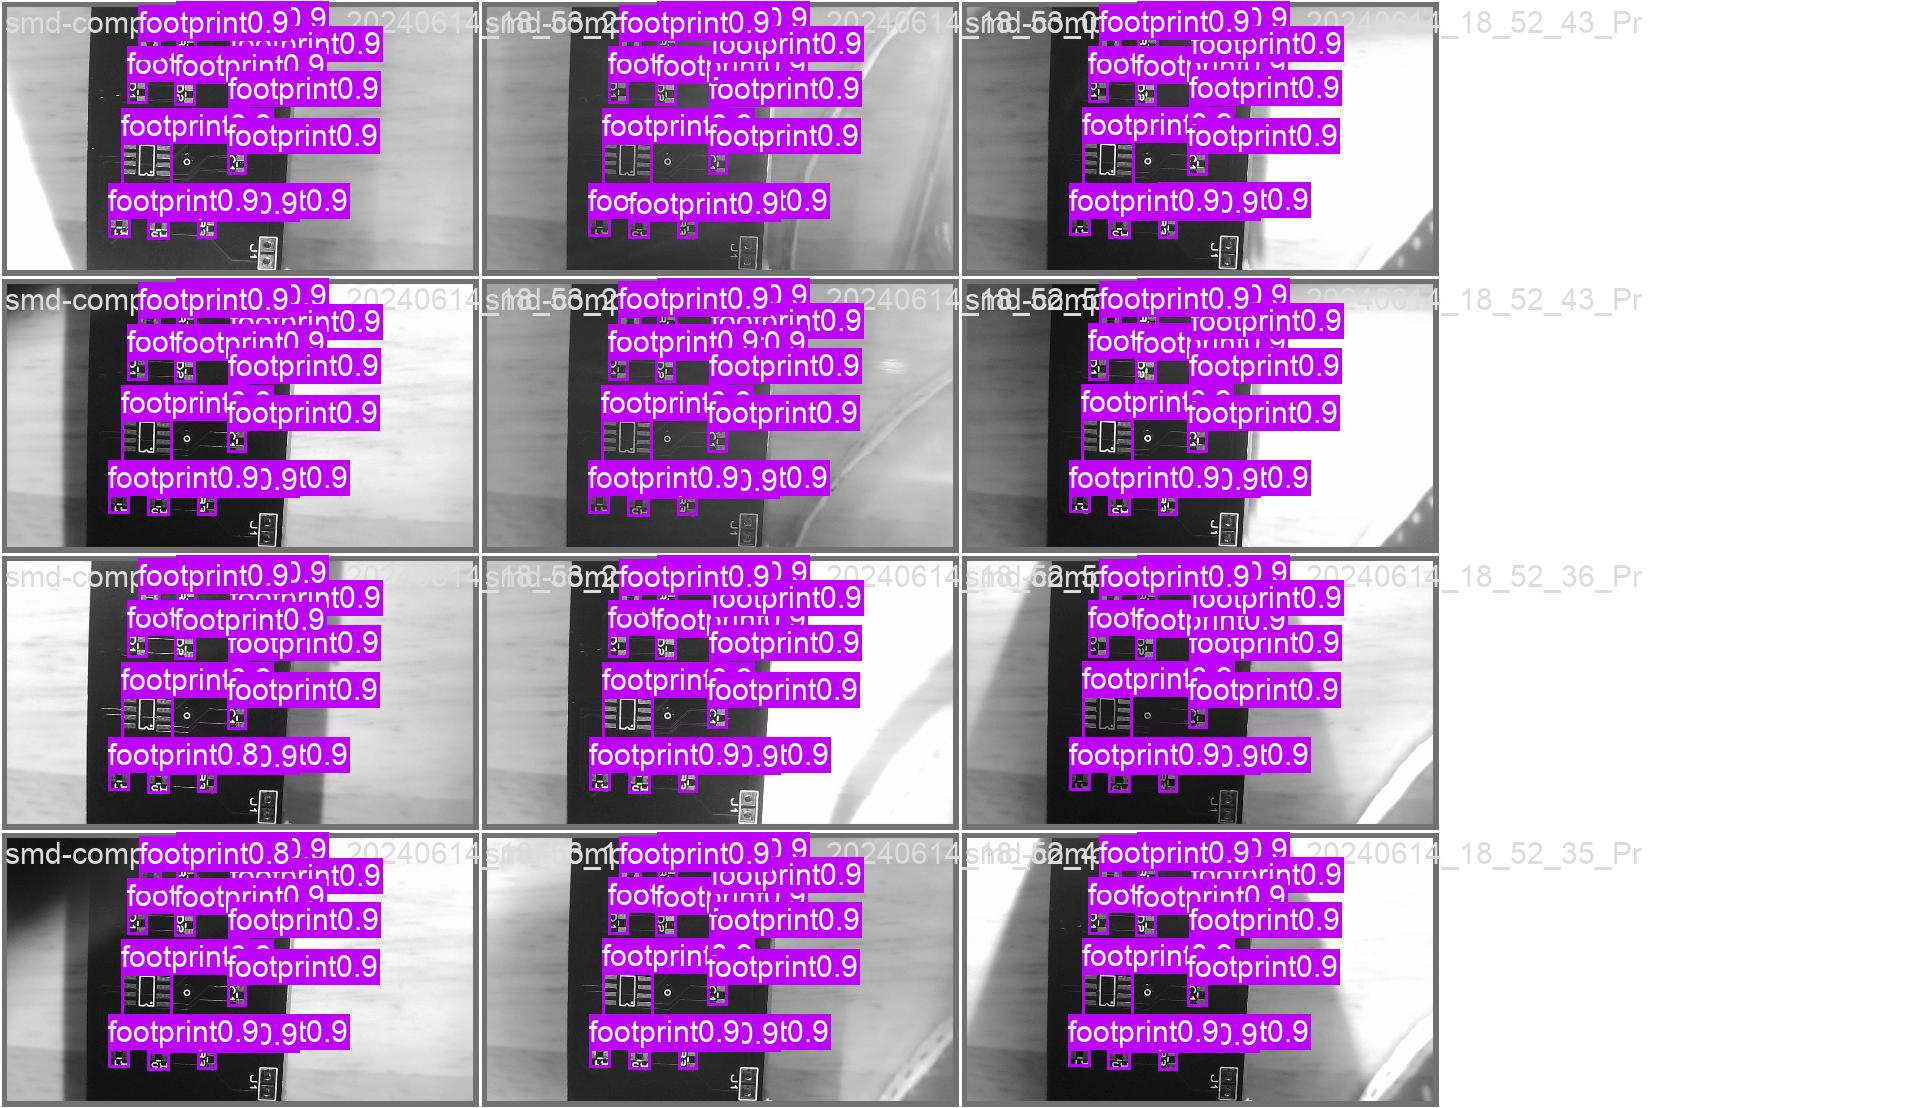
\includegraphics[width=0.85\textwidth]{figures/val_batch0_pred.jpg}
\caption{Пример предсказаний на валидационном батче (публичные/смешанные
кадры; часто footprint с высокой уверенностью).}
\label{fig:valpred}
\end{figure}

\subsection{Оценка по источникам и стенду}
\begin{table}[H]
\centering
\caption{mAP детектора det\_v0 по источникам (\texttt{eval.md})}
\label{tab:nn-map}
\begin{tabular}{@{}lcc@{}}
\toprule
Источник & mAP50 & mAP50-95 \\
\midrule
synth & \textbf{0{,}932} & 0{,}891 \\
public & 0{,}381 & 0{,}258 \\
\bottomrule
\end{tabular}
\end{table}

На публичных фото сильны \texttt{led}/\texttt{footprint}/\texttt{ic},
слабы мелкие R/C/diode/inductor (типичный domain gap).

\begin{table}[H]
\centering
\caption{Целые кадры новых синтетических дизайнов: recall позиции и класс}
\label{tab:nn-bench}
\begin{tabular}{@{}lrrr@{}}
\toprule
Класс & позиций & найдено & верный класс \\
\midrule
capacitor & 156 & 100{,}0\,\% & 98{,}7\,\% \\
resistor & 112 & 100{,}0\,\% & 99{,}1\,\% \\
ic & 41 & 100{,}0\,\% & 100{,}0\,\% \\
diode & 31 & 100{,}0\,\% & 100{,}0\,\% \\
transistor & 27 & 100{,}0\,\% & 100{,}0\,\% \\
led & 15 & 100{,}0\,\% & 100{,}0\,\% \\
electrolytic & 12 & 100{,}0\,\% & 100{,}0\,\% \\
footprint & 12 & 83{,}3\,\% & 75{,}0\,\% \\
inductor & 10 & 100{,}0\,\% & 100{,}0\,\% \\
crystal & 5 & 100{,}0\,\% & 100{,}0\,\% \\
\midrule
\multicolumn{4}{@{}l@{}}{Дефекты: missing \(12\to 91{,}7\,\%\); wrong \(6\to 100\,\%\).
Время \(\approx 0{,}36\,\mathrm{s}/\)кадр (тайлы 1024).} \\
\bottomrule
\end{tabular}
\end{table}

Интерпретация для статьи: на \emph{своей} синтетике детектор почти идеален;
на чужих фото --- нет. Это аргумент \emph{за} CAD+golden как основной контур
и \emph{против} заявки <<NN AOI готов к линии>> без реальной камеры и домена.

%--------------------------------------------------------------------------
\section{Ограничения и границы применимости}
\label{sec:limits}
%--------------------------------------------------------------------------

\begin{itemize}[leftmargin=1.5em]
  \item Не покрыто: объём галтели, lifted lead, подкорпусные BGA/QFN, цвет,
        OCR маркировки.
  \item Камерные бэкенды не подтверждены на железе.
  \item Стенд процедурный: полезен для регрессии алгоритма, не заменяет
        линию.
  \item Цель false positions \(<0{,}2\,\%\) ещё не достигнута.
\end{itemize}

%--------------------------------------------------------------------------
\section{Дальнейшая работа}
\label{sec:future}
%--------------------------------------------------------------------------

\begin{enumerate}[leftmargin=1.5em]
  \item Косой / многоракурсный свет для сколов на верхней грани.
  \item OCR для wrong-IC / marking.
  \item Снижение FP: больше golden, адаптация \(\sigma\) под партию~B.
  \item Fine-tune детектора на реальных кадрах стенда.
  \item Bring-up Basler/Hikrobot; перенос дисциплины камеры/калибровки
        в смежный проект склада (\texttt{sklad-digital-twin}).
\end{enumerate}

%--------------------------------------------------------------------------
\section{Заключение}
%--------------------------------------------------------------------------

Показан рабочий CAD-управляемый классический AOI-прототип на OpenCV:
выравнивание, окна с параллаксом, статистическая golden-модель с зонами
корпуса, измеримые признаки дефектов и отчётность. На синтетическом стенде
v6 достигает \(93{,}3\,\%\) обнаружения и \(87{,}6\,\%\) верного класса при
\(0\,\%\) пропуска брака как PASS; зональная модель устраняет катастрофические
ложные на новой партии. Опциональный YOLO11s подтверждает сильный synth
mAP и слабый public mAP --- полезен как гипотеза second opinion, но не
заменяет метрологический контур при наличии CAD и контролируемого света.

%--------------------------------------------------------------------------
\section*{Чеклист для правки под требования редакции}
%--------------------------------------------------------------------------
\begin{itemize}[leftmargin=1.5em]
  \item Язык (RU/EN), шаблон журнала/конференции, лимит страниц.
  \item Нумерация формул/рисунков, стиль ссылок (GOST / IEEE / BibTeX).
  \item Нужны ли анонимизация, ORCID, ключевые слова, UDC.
  \item Какие фигуры обязательны (блок-схема пайплайна, схема оптики,
        кропы PASS/FAIL) --- сейчас заготовки из \texttt{nn\_results} и
        preview стенда.
  \item Политика цитирования промышленных систем (HALCON и др.) --- смягчить
        формулировки <<в духе>> vs прямые сравнения.
\end{itemize}

\begin{thebibliography}{9}
\bibitem{opencv}
  Bradski G. The OpenCV Library. \textit{Dr.\ Dobb's Journal}, 2000.
\bibitem{yolo11}
  Ultralytics. YOLO11 documentation.
  \url{https://docs.ultralytics.com/}
\bibitem{halcon}
  MVTec Software. HALCON --- Machine Vision Algorithms (variation model /
  matching concepts). Product documentation.
\bibitem{repo}
  Iliukhin I. aoi-micro. GitHub repository.
  \url{https://github.com/f1b0nacc1-afk/aoi-micro}
\end{thebibliography}

\end{document}
